\section{Neural Network Architecture}
\label{sec:nn-arch}

Our neural network architecture consists of a feature extraction (FE) block and a posterior estimation (PE) block, as shown in Fig.~\ref{fig:nn-arch}. The FE block learns to extract key features from the image, spectra, and metadata of a galaxy, and condenses them into a 1D feature vector. The feature vector is then used as the condition for the PE block to estimate the posterior of our galaxy parameters. We describe each block in detail below.

\begin{table*}
    \centering
    \begin{tabular}{l l l}
    \toprule
    \textbf{Branch} &
    \parbox[t]{14.5cm}{\raggedright \textbf{Architecture description}} &
    \textbf{Output} \\
    \tableline
    \addlinespace[5pt]

    Image &
    \parbox[t]{14.5cm}{\raggedright Two 3$\times$3 convolutions at 64 channels, each with BatchNorm and ReLU; 3$\times$3 stride-2 max pool; four 128-channel residual blocks with downsampling in the fourth; five 256-channel residual blocks with downsampling in the fifth; five 512-channel residual blocks with downsampling in the fifth; final 3$\times$3 average pool} &
    512 \\ \addlinespace[5pt]

    Spectra &
    \parbox[t]{14.5cm}{\raggedright Pairs of 3$\times$3 convolutions at 16, 32, 64, and 128 channels, each convolution followed by BatchNorm and ReLU; 1$\times$2 max pooling along wavelength after the 16- and 32-channel pairs; two 256-channel 3$\times$3 convolutions; final 5$\times$16 convolution spanning all fibers and remaining wavelength bins} &
    512 \\ \addlinespace[5pt]

    Metadata &
    \parbox[t]{14.5cm}{\raggedright Concatenate ten fiber coordinates with $m_r$, $\rho_I$, and $\rho_S$; linear layers $13 \to 64 \to 128$, each followed by GELU, then LayerNorm} &
    128 \\ \addlinespace[5pt]

    \tableline
    \end{tabular}
    \caption{Description of the architecture of each branch in the feature extraction block.}
    \label{tab:fe-desc}
\end{table*}

\begin{figure*}
    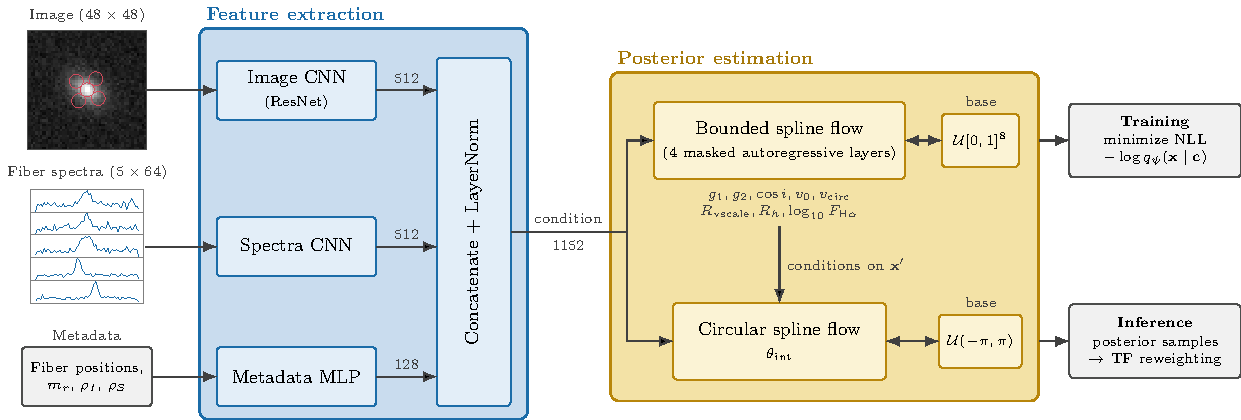
\includegraphics[width=\linewidth]{figs/nn_arch.pdf}
    \caption{Schematic of our neural network model. The image, spectra, and metadata of a galaxy are processed separately by the three branches of the feature extraction block (Table~\ref{tab:fe-desc}), whose outputs are concatenated into a 1152-dimensional feature vector. This vector is used as the condition for the normalizing flow in the posterior estimation block (Sec.~\ref{ssec:npe}), which consists of a bounded spline flow for the eight parameters that have a finite range, and a circular spline flow for $\theta_\mathrm{int}$ to account for its cyclic nature. The feature extraction block is pretrained with a contrastive loss (Sec.~\ref{ssec:pretrain}) and then kept fixed, while the flow is trained by minimizing the negative log-likelihood of the true parameters. During inference, we draw posterior samples from the flow and reweigh them by the TF prior (Sec.~\ref{ssec:tf-prior}). The example image and spectra are from a galaxy in the Xu3 test set, with its five fiber positions marked on the image in red.}
    \label{fig:nn-arch}
\end{figure*}

\subsection{Feature Extraction with Convolutional Networks}
\label{ssec:feature-extract}
Our FE block consists of a branched, convolutional neural network (CNN)-based architecture \citep{cnn} where one branch processes the image, one processes the spectra, and a third small branch processes the metadata (see Table~\ref{tab:fe-desc}).

The image branch first expands the data to 64 channels through two convolution layers, before applying a max pooling layer to reduce the image dimensions by half. It is then processed through a residual network (ResNet) \citep{resnet}, consisting of 2-layer residual blocks where the input of the block is added back to its output. This is a well-known structure that works well in extracting features from high-dimensional data forms such as images. We use 14 blocks, or 28 residual layers, for the ResNet. The 14 blocks consist of 3 sections of 4-5 blocks, where we double the number of channels in the first block of every section and halve the image dimensions in the last block. In the final layer, we use an average pooling layer to reduce the image dimensions to $1\times1$, giving us a 1D feature vector of 512 channels. Batch normalization is applied after every convolution layer.

For the spectra, we treat the five fiber spectra of a galaxy as a single $5\times64$ image, with fibers along one axis and wavelength along the other, so that the convolutions can learn features between fibers as well as along wavelengths. The spectra branch consists of pairs of convolution layers at 16, 32, 64, and 128 channels, followed by two convolution layers at 256 channels. After each of the first two pairs, we apply a max pooling layer that halves the number of wavelength bins, reducing them from 64 to 16. The final convolution layer has a kernel that spans all five fibers and the remaining 16 wavelength bins, which combines the information from all fibers into a 1D feature vector of 512 channels. As is the case for the image branch, every convolution layer is followed by batch normalization.

The metadata branch is a small multi-layer perceptron (MLP) that maps the ten fiber coordinates and the three values of $m_r$, $\rho_I$, and $\rho_S$ (Sec.~\ref{ssec:datasets}) into a 128-dimensional feature vector. Finally, the outputs of the three branches are concatenated into a single 1152-dimensional feature vector, which is normalized with a LayerNorm before being passed to the PE block as its condition.

\subsection{Contrastive Pretraining for the Feature Extractor}
\label{ssec:pretrain}
Before training the PE block, we pretrain the FE block using contrastive learning. The goal of contrastive learning, in general, is to achieve a diverse and properly distributed embedding space by bringing embedding vectors of similar data closer and pushing those of very different data further \citep{SimCLR, SupCon}. In our case, we consider two galaxies similar if their KL parameters are close in parameter space. Since our parameters change continuously rather than discretely, we implement a continuous version of the supervised contrastive loss of \citep{SupCon}, in which each pair of galaxies is weighted by how close their parameters are. We therefore refer to this learning scheme as continuous contrastive learning (CCL). Comparing between small-scale training runs with pretraining and one without, we found that the pretrained model achieves about 2\% less shape noise when evaluated on the same test set, and gives better-calibrated posteriors of $\theta_\mathrm{int}$. Pretraining also has the practical advantage of compartmentalizing the training process, such that one can modify the latter blocks without having to train an entire model from scratch.

For pretraining, we attach a projection head to the end of the FE block, which is an MLP with layer sizes $1152 \to 2048 \to 512 \to 128$. The output from it is normalized to unit length, giving us an embedding $\mathbf{u}_i$ for each galaxy $i$ in a batch. For two galaxies $i$ and $j$, we measure the distance between their parameters as
\begin{equation}
\label{eqn:ccl-distance}
    d_{ij}^2 = \frac{1}{9}\sum_{k=1}^{9}\left(\tilde{\theta}_{ik} - \tilde{\theta}_{jk}\right)^2,
\end{equation}
where $\tilde{\theta}_{ik}$ is the $k$-th parameter of galaxy $i$, rescaled to $[-1, 1]$ using the ranges in Table~\ref{tab:kl-params}. Since $\theta_\mathrm{int}$ is a cyclic parameter, we take its difference around the circle. We then normalize the weights, including a background term $w_\mathrm{bg}$, into target weights $t_{ij}$:
\begin{equation}
\label{eqn:ccl-target}
    w_{ij} = \exp\left(-\frac{d_{ij}^2}{2\sigma_d^2}\right), \qquad
    t_{ij} = \frac{w_{ij}}{\sum_{k\neq i} w_{ik} + w_\mathrm{bg}},
\end{equation}
where $\sigma_d = 0.15$ sets the sharpness of the weight function, i.e. how close two galaxies need to be to count as similar. The background term, $w_\mathrm{bg} = \exp\left(-d_\mathrm{cut}^2/2\sigma_d^2\right)$, with $d_\mathrm{cut}=0.4$, is a cutoff distance that ensures that a galaxy sufficiently far from every other galaxy in the batch does not have a significant impact on the loss. Our loss function is
\begin{equation}
\label{eqn:ccl-loss}
    \mathcal{L}_\mathrm{CCL} = -\frac{1}{N}\sum_{i=1}^{N}\sum_{j\neq i} t_{ij}\log\frac{\exp(\mathbf{u}_i\cdot\mathbf{u}_j/T)}{\sum_{k\neq i}\exp(\mathbf{u}_i\cdot\mathbf{u}_k/T)},
\end{equation}
where $T=0.1$ is a temperature parameter and $N$ is the number of galaxies in the batch. This loss achieves our goal with contrastive learning, where its value is small when the embeddings of galaxies with similar parameters point in similar directions, and large otherwise. Each galaxy appears in its batch twice, once as simulated and once rotated by $90\degree$, with its parameters transformed accordingly (Sec.~\ref{ssec:npe}). All hyperparameters for the pretraining ($\sigma_d$, $d_\mathrm{cut}$ and $T$) are pre-selected from physical intuition, and then tested empirically through short training tests, and we do not claim our choices to be optimal. After pretraining, we discard the projection head and use the frozen weights of the pretrained FE block to train the PE block. Only the LayerNorm layer at the end of the FE block is trained together with the PE block.

\subsection{Posterior Estimation with Normalizing Flows}
\label{ssec:npe}
After we have extracted features from the data, we would like to estimate the posterior distributions of the KL parameters. A good architectural choice for this is a conditional normalizing flow (CNF) \citep{NormalizingFlows, CNF}. CNFs are commonly used in NPE, and have a simpler implementation than other choices like VAEs, GANs or diffusion models, while being much more flexible and expressive than a multi-layer perceptron (MLP).

To explain briefly, a CNF learns a bijective mapping $f_\psi$ between a target distribution $p_x(\mathbf{x \mid c})$ and a simple base distribution $p_z(\mathbf{z})$, where $\mathbf{c}$ is a condition vector and $\psi$ are the parameters of the network:
\begin{equation}
\label{eqn:cnf-transform}
    \mathbf{z} = f_\psi(\mathbf{x}; \mathbf{c}); \qquad \mathbf{x} = f_\psi^{-1}(\mathbf{z}; \mathbf{c}).
\end{equation}
In our case, the target distribution is the posterior of the KL parameters, and the condition is the feature vector from the FE block. By change of variables, we can express the probability density of $\mathbf{x}$ in terms of the base distribution:
\begin{equation}
\label{eqn:cnf-cv}
    q_\psi(\mathbf{x \mid c}) = p_z\left(f_\psi(\mathbf{x}; \mathbf{c})\right) \cdot \left| \det\left(\frac{\partial f_\psi(\mathbf{x}; \mathbf{c})}{\partial\mathbf{x}}\right)\right| ,
\end{equation}
where the $ |\det(\cdot)| $ term is the Jacobian determinant of $f_\psi(\mathbf{x}; \mathbf{c})$. This formulation allows us to compute the probability of the true KL parameters of each training galaxy conditioned on its features, from which we compute our loss function, the negative log-likelihood (NLL):
\begin{equation}
\label{eqn:loss-unweighted}
    \mathcal{L}(\psi) = -\frac{1}{N}\sum_{i=1}^N\log q_\psi(\mathbf{x}_i \mid \mathbf{c}_i).
\end{equation}
After training, we can draw posterior samples for any galaxy by drawing $\mathbf{z}$ from the base distribution and passing it through the inverse mapping $f_\psi^{-1}$.

A common choice for the base distribution is a standard Gaussian, which assigns some probability to every value of $\mathbf{x}$. However, all of our parameters have a finite range set by the training prior (Table~\ref{tab:kl-params}), and $\theta_\mathrm{int}$ is cyclic. We design our flow to respect both of these properties. For the eight parameters other than $\theta_\mathrm{int}$, which we denote as $\mathbf{x}'$, we rescale each parameter to $[0, 1]$ using its prior range, and use a uniform base distribution on the unit box $[0, 1]^8$. The mapping between them is made of rational-quadratic spline (RQS) transforms \citep{NeuralSplineFlows}, which map the interval $[0,1]$ onto itself, so that the learned posterior is exactly zero outside of the prior range. For $\theta_\mathrm{int}$, we use a circular RQS \citep{FlowsToriSpheres}, which keeps the density continuous across $\theta_\mathrm{int}=\pm\pi$. The joint posterior is then written as
\begin{equation}
\label{eqn:flow-factorization}
    q_\psi(\mathbf{x} \mid \mathbf{c}) = q_\psi(\mathbf{x}' \mid \mathbf{c})\, q_\psi(\theta_\mathrm{int} \mid \mathbf{x}', \mathbf{c}),
\end{equation}
where the distribution of $\theta_\mathrm{int}$ is conditioned on both the features and the other eight parameters, so that the correlations between them can still be learned by the flow.

The flow for $\mathbf{x}'$ consists of 4 masked autoregressive spline layers \citep{MAF, NeuralSplineFlows}, where the transformation of each parameter depends only on the parameters before it. This is vital for computational efficiency, as it gives us a triangular Jacobian matrix, whose determinant is simply the product of its diagonal terms. The spline parameters of each layer are predicted from $\mathbf{c}$ and the preceding parameters by a MADE (Masked Autoencoder for Distribution Estimation) network \citep{MADE} with 256 hidden units and 2 residual blocks, and each spline has 8 bins. We reverse the order of the parameters between layers, which is common practice when training normalizing flows, so that every parameter can depend on every other parameter. The flow for $\theta_\mathrm{int}$ is a single circular spline with 8 bins, whose parameters are predicted by an MLP with two hidden layers of 128 units from $\mathbf{c}$ and $\mathbf{x}'$. We implement our flow using the \texttt{nflows} package \citep{nflows} as a foundation.

The CNF in itself does not directly minimize shear bias, but in modern cosmic shear surveys, we typically require additive biases of a shear measurement method to be very small $(<10^{-4})$ or consistent with zero [cite DES, HSC and others]. To ensure that our model does not acquire a significant additive bias, we make our model symmetric under $90\degree$ rotations. Rotating a galaxy by $90\degree$ flips the sign of both shear components, $(g_1, g_2) \rightarrow (-g_1, -g_2)$, and shifts its position angle by $\pi/2$. Its spectra stay the same, since our fibers are placed relative to the galaxy's own axes (Sec.~\ref{ssec:kl-model}). During training, each datavector shown to the model has a $50\%$ chance of being rotated by 90 degrees. This ensures that the model learns equally from each shear pair and its opposite. During inference, we pass both the original and the rotated datavectors through the model, rotate the latter's posterior draws back to the original frame, and combine the samples. This way, any constant offset in shear that the model might learn, e.g. from a preferred direction on the pixel grid, cancels out between them. While this double treatment in both training and inference may seem redundant, we have found through small training tests that both are necessary, and applying only one treatment gives us additive biases of $\sim7-30 \sigma$ significance $(\sigma\approx1.4*10^{-4})$. Applying both treatments reduces the additive bias in both components to $<1\sigma$, which is consistent with zero. It should be noted that this procedure does not significantly add to training or inference time. During training, we are not passing extra batches, but only augmenting $\sim50\%$ of each batch. Inference time is dominated by sampling rather than forward passes of the data, and we allocate half of our samples to the identity and the other half to the rotated data, so that our total number of samples stays the same.

\subsection{Incorporating the TF Prior}
\label{ssec:tf-prior}
As shown in Sec.~\ref{sec:kl-basics}, we need a constraint on $\vcirc$ from the TFR in order to break the degeneracy between intrinsic shape and shear. However, we sample $\vcirc$ uniformly in our training set (Table~\ref{tab:kl-params}), so the posteriors learned by our model correspond to a uniform prior on $\vcirc$. Instead of building the TFR into training, we apply it after training by reweighting the posterior samples. If our model approximates the posterior under the training prior $\pi_\mathrm{train}$, the posterior under the TF prior $\pi_\mathrm{TF}$ is
\begin{equation}
\label{eqn:tf-reweight}
    p_\mathrm{TF}(\mathbf{x} \mid \mathbf{c}) \propto q_\psi(\mathbf{x} \mid \mathbf{c})\, \frac{\pi_\mathrm{TF}(\vcirc \mid m_r)}{\pi_\mathrm{train}(\vcirc)},
\end{equation}
while all other parameters keep their training priors. For each galaxy, we therefore give each posterior sample $\mathbf{x}_j$ a weight
\begin{equation}
\label{eqn:tf-weights}
    w_j = \frac{\pi_\mathrm{TF}(v_{\mathrm{circ},j} \mid m_r)/\pi_\mathrm{train}(v_{\mathrm{circ},j})}{\sum_k \pi_\mathrm{TF}(v_{\mathrm{circ},k} \mid m_r)/\pi_\mathrm{train}(v_{\mathrm{circ},k})},
\end{equation}
and compute all posterior summaries, such as the mean and credible intervals, with these weights. Essentially, we are applying importance sampling to the posterior samples, weighing more heavily the samples whose $\vcirc$ is more likely according to the TF prior. Since $\pi_\mathrm{train}(\vcirc)$ is uniform, the weights are simply proportional to the TF prior. Reweighting reduces the effective number of samples of each posterior, which we measure as $1/\sum_j w_j^2$. On the Xu3 test set (Sec.~\ref{ssec:test-set}), the median galaxy keeps 60\% of its $10^4$ samples, and 99.6\% of galaxies keep more than 1000, so the reweighted posteriors are well sampled for almost all galaxies. A benefit of this approach is that the TFR can be changed without retraining our model, e.g. when it is recalibrated on a new galaxy sample.

Our TF prior is a Gaussian in $\log_{10}\vcirc$, truncated to the training range of 60--540 km s$^{-1}$, with mean
\begin{equation}
\label{eqn:tf-mean}
    \langle\log_{10}\vcirc\rangle = \frac{36 - m_r}{7.22}
\end{equation}
and a standard deviation of $\sigma_\mathrm{TF}=0.1$ dex. In terms of Eq.~(\ref{eqn:TFR}), this corresponds to $a = 36/7.22$ and $b = -1/7.22$ mag$^{-1}$, with $m_r$ in place of $M$. Since all of our galaxies are simulated at the same redshift, we write the relation in terms of the apparent magnitude $m_r$. We assume a TFR slope of $-7.22$ mag per dex, which is the result of \citep{DESIPVTF2025}, and assume an intercept of 36 mag, which has been empirically chosen to cover a realistic range of $\vcirc$ across a realistic range of $m_r$. Our scatter of 0.1 dex is more conservative than measured intrinsic scatters in literature, such as 0.036 dex from \citep{Reyes11}, or 0.466 mag ($\approx$0.065 dex) from \citep{DESIPVTF2025}. Part of the reason for this is to account for the extra uncertainty from the measurement of $m_r$, since we treat $m_r$ as perfectly known in our model and do not add a separate magnitude uncertainty to the scatter. \XW{DESI/LS catalogs provide the inverse variance of the $r$-band flux, so we could eventually propagate the $m_r$ uncertainty of each galaxy into its TF scatter instead.} The same TFR is used to draw $\vcirc$ for our test sets (Sec.~\ref{ssec:test-set}).

\subsection{Training Configurations}
\label{ssec:train-conf}
We pretrain the FE block by minimizing the loss in Eq.~(\ref{eqn:ccl-loss}), using the AdamW optimizer \citep{AdamW} with a learning rate of $10^{-3}$ and a weight decay of $10^{-4}$. The learning rate is warmed up linearly from 1\% of its initial value over the first 5 epochs, and then lowered following a cosine schedule down to $10^{-6}$. We pretrain for 100 epochs with a batch size of 400, and keep the epoch with the lowest validation loss. Pretraining took about 1 hour on 4 NVIDIA V100 GPUs.

We then train the PE block by minimizing the NLL in Eq.~(\ref{eqn:loss-unweighted}), again with AdamW, with a weight decay of $10^{-5}$. We use an initial learning rate of $3\times10^{-4}$ for most of the PE block, and a lower learning rate of $10^{-4}$ for the flow of $\theta_\mathrm{int}$. The learning rate is warmed up linearly from 10\% of its initial value over the first 2 epochs, and then decreased following a cosine schedule down to $10^{-5}$ at the end of training. We also clip the norm of the gradients at 1 to stabilize training. We use a batch size of 400, split across 4 NVIDIA V100 GPUs. We train for up to 200 epochs, stopping early if the validation loss does not improve by more than $10^{-3}$ for 20 epochs, and pick the epoch with the lowest validation loss for testing. Training the PE block also took about 1 hour on 4 NVIDIA V100 GPUs. \XW{These numbers are from the current model trained on 100k galaxies. Will update them for the 1M model.}
